\section{Séance 2}
\subsection{Parcours fermés} Dans le graphe ci-dessous, trouvez le nombre de parcours fermés de longueur $k$ contenant le point $A$.

\begin{figure}[h!]
  \begin{center}
    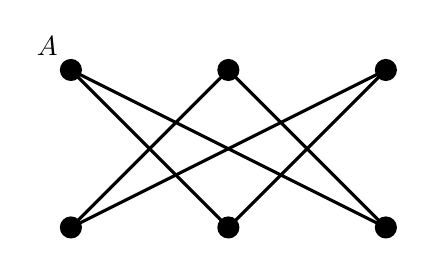
\begin{tikzpicture}[scale=1,looseness=1,auto,line width=.4mm]

      \path[draw=none] (-2.3,1.3) node { $A$ };

      \draw (-2, 1) -- ( 0,-1);
      \draw (-2, 1) -- ( 2,-1);
      \draw ( 0, 1) -- (-2,-1);
      \draw ( 0, 1) -- ( 2,-1);
      \draw ( 2, 1) -- (-2,-1);
      \draw ( 2, 1) -- ( 0,-1);

      \draw[fill=black] (-2,-1) circle(.12);
      \draw[fill=black] (-2, 1) circle(.12);
      \draw[fill=black] ( 0,-1) circle(.12);
      \draw[fill=black] ( 0, 1) circle(.12);
      \draw[fill=black] ( 2,-1) circle(.12);
      \draw[fill=black] ( 2, 1) circle(.12);

    \end{tikzpicture}
  \end{center}
\end{figure}

\begin{solution}
On cherche le nombre de parcours fermé partant de A de longueur $k$.
Pour cela, on utilise le théorème suivant :

$\,$

Soit $A$ la matrice d'adjacence d'un graphe. Alors l'élément $ij$
de $A^{k}$ ($k\geq0$) est le nombre de parcours de longueur $k$
de $v_{i}$ vers $v_{j}$.

$\,$

Dans notre cas, le graphe est biparti non complet et la matrice d'adjacence
est donnée par :

\[
A=\left(\begin{array}{cccccc}
0 & 0 & 0 & 0 & 1 & 1\\
0 & 0 & 0 & 1 & 0 & 1\\
0 & 0 & 0 & 1 & 1 & 0\\
0 & 1 & 1 & 0 & 0 & 0\\
1 & 0 & 1 & 0 & 0 & 0\\
1 & 1 & 0 & 0 & 0 & 0
\end{array}\right)
\]


Si $k$ est impair, la matrice d'adjacence élevée à la puissance $k$
deviendra :

\[
A^{k}=\left(\begin{array}{cc}
\begin{array}{ccc}
0 & 0 & 0\\
0 & 0 & 0\\
0 & 0 & 0
\end{array} & \left[\begin{array}{ccc}
0 & 1 & 1\\
1 & 0 & 1\\
1 & 1 & 0
\end{array}\right]^{k}\\
\left[\begin{array}{ccc}
0 & 1 & 1\\
1 & 0 & 1\\
1 & 1 & 0
\end{array}\right]^{k} & \begin{array}{ccc}
0 & 0 & 0\\
0 & 0 & 0\\
0 & 0 & 0
\end{array}
\end{array}\right)
\]


Comme on cherche des parcours fermé de A vers A, on s'intéresse uniquement
aux éléments diagonaux qui sont, dans le cas où $k$ est impair, tous
nuls. Par conséquent, le nombre de parcours fermé de longueur $k$
vaut 0.

Si $k$ est pair, la matrice d'adjacence élevée à la puissance $k$
deviendra :

\[
A^{k}=\left(\begin{array}{cc}
\left[\begin{array}{ccc}
0 & 1 & 1\\
1 & 0 & 1\\
1 & 1 & 0
\end{array}\right]^{k} & \begin{array}{ccc}
0 & 0 & 0\\
0 & 0 & 0\\
0 & 0 & 0
\end{array}\\
\begin{array}{ccc}
0 & 0 & 0\\
0 & 0 & 0\\
0 & 0 & 0
\end{array} & \left[\begin{array}{ccc}
0 & 1 & 1\\
1 & 0 & 1\\
1 & 1 & 0
\end{array}\right]^{k}
\end{array}\right)
\]


Dans ce cas, les éléments diagonaux de $A^{k}$ sont non nuls. De
plus, les sous-blocs $\left[\begin{array}{ccc}
0 & 1 & 1\\
1 & 0 & 1\\
1 & 1 & 0
\end{array}\right]^{k}$correspondent à une matrice d'adjacence élevée à la puissance $k$
d'un graphe complet. Dans la première séance d'exercice, on a démontré
une formule pour calculer une entrée de la diagonale de cette matrice
:

\[
\#\, parcours\, ferm\acute{e}\, de\, longueur\, k\, de\, A\rightarrow A=\frac{(n-1)}{n}((n-1)^{k-1}+(-1)^{k})
\]


Ici $k$ est pair, donc $(-1)^{k}=1$ et $n=3$ (sous-blocs), on obtient
:

\[
\#\, parcours\, ferm\acute{e}\, de\, longueur\, k\, de\, A\rightarrow A=\frac{2}{3}(2{}^{k-1}+1)
\]
\end{solution}

\subsection{Tracer d'un coup} Est-il possible de tracer les figures suivantes sans lever le crayon et sans passer deux fois par le même segment?

\begin{figure}[h!]
  \begin{center}
    \begin{tabular}{lcccr}
      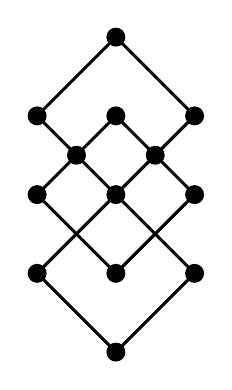
\begin{tikzpicture}[scale=1,looseness=1,auto,line width=.4mm]

        \draw (-1, 1) -- (  0, 2);
        \draw (-1, 1) -- (-.5,.5);
        \draw (-1, 0) -- (  0,-1);
        \draw (-1, 0) -- (-.5,.5);
        \draw (-1,-1) -- (  0, 0);
        \draw (-1,-1) -- (  0,-2);
        \draw ( 1, 1) -- (  0, 2);
        \draw ( 1, 1) -- ( .5,.5);
        \draw ( 1, 0) -- (  0,-1);
        \draw ( 1, 0) -- ( .5,.5);
        \draw ( 1,-1) -- (  0, 0);
        \draw ( 1,-1) -- (  0,-2);
        \draw ( 0, 0) -- ( .5,.5);
        \draw ( 0, 0) -- (-.5,.5);
        \draw ( 0, 1) -- ( .5,.5);
        \draw ( 0, 1) -- (-.5,.5);

        \draw[fill=black] ( -1, 1) circle(.1);
        \draw[fill=black] ( -1, 0) circle(.1);
        \draw[fill=black] ( -1,-1) circle(.1);
        \draw[fill=black] (  0,-2) circle(.1);
        \draw[fill=black] (  0,-1) circle(.1);
        \draw[fill=black] (  0, 0) circle(.1);
        \draw[fill=black] (  0, 1) circle(.1);
        \draw[fill=black] (  0, 2) circle(.1);
        \draw[fill=black] (  1, 1) circle(.1);
        \draw[fill=black] (  1, 0) circle(.1);
        \draw[fill=black] (  1,-1) circle(.1);
        \draw[fill=black] (-.5,.5) circle(.1);
        \draw[fill=black] ( .5,.5) circle(.1);

      \end{tikzpicture}
      & \hspace{1cm} &
      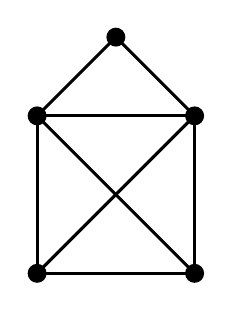
\begin{tikzpicture}[scale=1,looseness=1,auto,line width=.4mm]

        \draw (0,0) -- (2,0);
        \draw (0,0) -- (2,2);
        \draw (0,0) -- (0,2);
        \draw (2,0) -- (2,2);
        \draw (2,0) -- (0,2);
        \draw (0,2) -- (2,2);
        \draw (0,2) -- (1,3);
        \draw (2,2) -- (1,3);

        \draw[fill=black] (0,0) circle(.1);
        \draw[fill=black] (2,0) circle(.1);
        \draw[fill=black] (2,2) circle(.1);
        \draw[fill=black] (0,2) circle(.1);
        \draw[fill=black] (1,3) circle(.1);

      \end{tikzpicture}
      & \hspace{1cm} &
      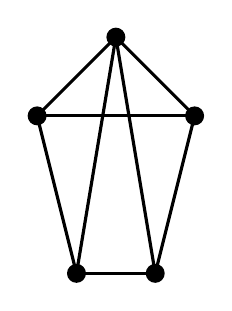
\begin{tikzpicture}[scale=1,looseness=1,auto,line width=.4mm]

        \draw (.5,0) -- (1.5,0);
        \draw (.5,0) -- (1,3);
        \draw (.5,0) -- (0,2);
        \draw (1.5,0) -- (2,2);
        \draw (1.5,0) -- (1,3);
        \draw (0,2) -- (2,2);
        \draw (0,2) -- (1,3);
        \draw (2,2) -- (1,3);

        \draw[fill=black] (.5,0) circle(.1);
        \draw[fill=black] (1.5,0) circle(.1);
        \draw[fill=black] (2,2) circle(.1);
        \draw[fill=black] (0,2) circle(.1);
        \draw[fill=black] (1,3) circle(.1);

      \end{tikzpicture}
    \end{tabular}
  \end{center}
\end{figure}

\begin{solution}
Tracer les figures sans lever le crayon et sans passer deux fois par
le même segment, revient à chercher un parcours eulérien :
\begin{itemize}
\item Tous les sommets sont de degré pair, par le théorème d'Euler on en
conclut que le graphe est eulérien. Il existe donc un parcours eulérien
fermé.
\item 2 noeuds sont de degré impair, on utilise le théorème suivant :
\end{itemize}
\begin{center}
\par Un graphe connexe possède un parcours eulérien ssi le nombre de noeuds de degré impair est zéro ou deux.

\end{center}

Il existe donc un parcours eulérien dans le premier et le deuxième.
Il y a 4 noeuds qui sont de degré impair dans le dernier, il n'existe donc pas de parcours eulérien.

\end{solution}

\subsection{Algorithme pour trouver un circuit eulérien} En vous basant sur la preuve inductive du théorème qui caractérise les graphes eulériens, décrivez un algorithme qui trouve un circuit eulérien en un temps $O(|E|)$.
\begin{solution}
Il faut utiliser la preuve du théorème d'Euler :

\begin{center}
Un graphe connexe est eulérien ssi tous les sommets sont de degré
pair
\par\end{center}

La deuxième partie de la preuve consiste en la construction d'un parcours
eulérien, cela nous donne aussi un algorithme pour trouver un parcours
eulérien.

Le principe de l’algorithme est simple:
\begin{itemize}
\item on prend un nœud non parcouru encore;
\item on prend les arêtes non parcourue encore jusqu'à revenir sur le noeud de départ;
\item on merge ce parcours avec ceux déjà trouver;
\item si il n'y a plus de nœud non exploré, on a fini. Sinon on reprend au point 1.
\end{itemize}
\end{solution}
\subsection{Séquences de de Bruijn.} Le problème suivant apparaît sous de nombreuses formes. On demande de construire la plus longue séquence circulaire de lettres d'un alphabet de $k$ lettres sans qu'aucune sous-séquence de longueur $n$ ne soit répétée.
\begin{enumerate}
  \item Donnez une borne supérieure sur la longueur de la séquence circulaire en question.
  \item Cette borne peut-elle être atteinte? Formulez cette question comme un problème de tour eulérien dans un graphe orienté. (Indice~: les sommets correspondent aux séquences de longueur $n-1$ et les arêtes aux séquences de longueur $n$.)
  \item Pour l'alphabet $\mathcal{A} = \{0, 1, 2\}$ de $k = 3$ lettres et pour $n = 3$, répondez à la question précédente en construisant la plus longue séquence circulaire.
\end{enumerate}
\begin{solution}
1. $k^{n}$ est une borne supérieure sur le nombre de sous-séquences
de longueur $n$. Puisqu'on ne peut pas les répéter, la plus longue
chaîne utilisera toutes les sous-séquences.

2.oui

3.
\end{solution}
\pagebreak
\subsection{Parcourt fermé de poid minimum} On souhaite trouver un parcours fermé de poids minimum passant au moins une fois par chaque arête du graphe suivant~:
\begin{figure}[h!]
  \begin{center}
    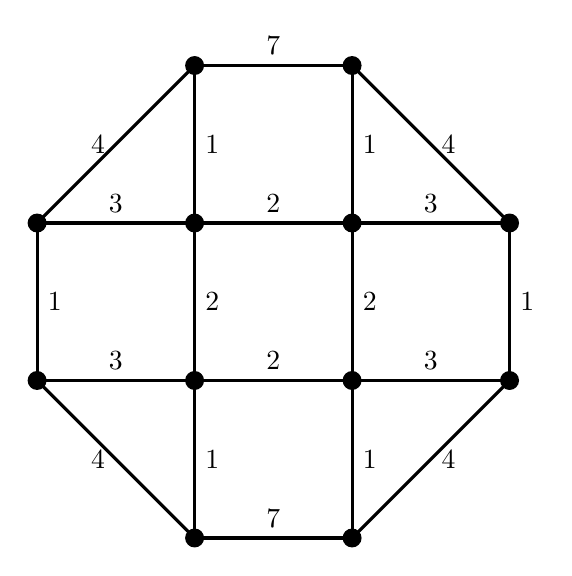
\begin{tikzpicture}[scale=1,auto,line width=.4mm]

      \coordinate (11++) at ( 1, 1);
      \coordinate (13++) at ( 1, 3);
      \coordinate (31++) at ( 3, 1);
      \coordinate (11+-) at ( 1,-1);
      \coordinate (13+-) at ( 1,-3);
      \coordinate (31+-) at ( 3,-1);
      \coordinate (11-+) at (-1, 1);
      \coordinate (13-+) at (-1, 3);
      \coordinate (31-+) at (-3, 1);
      \coordinate (11--) at (-1,-1);
      \coordinate (13--) at (-1,-3);
      \coordinate (31--) at (-3,-1);

      \draw (11++) -- (13++) node[midway,right] {$1$};
      \draw (11++) -- (31++) node[midway,above] {$3$};
      \draw (31++) -- (13++) node[midway,above,right] {$4$};
      \draw (11+-) -- (13+-) node[midway,right] {$1$};
      \draw (11+-) -- (31+-) node[midway,above] {$3$};
      \draw (31+-) -- (13+-) node[midway,below,right] {$4$};
      \draw (11-+) -- (13-+) node[midway,right] {$1$};
      \draw (11-+) -- (31-+) node[midway,above] {$3$};
      \draw (31-+) -- (13-+) node[midway,above,left] {$4$};
      \draw (11--) -- (13--) node[midway,right] {$1$};
      \draw (11--) -- (31--) node[midway,above] {$3$};
      \draw (31--) -- (13--) node[midway,below,left] {$4$};
      \draw (11++) -- (11+-) node[midway,right] {$2$};
      \draw (11++) -- (11-+) node[midway,above] {$2$};
      \draw (11--) -- (11+-) node[midway,above] {$2$};
      \draw (11--) -- (11-+) node[midway,right] {$2$};
      \draw (13++) -- (13-+) node[midway,above] {$7$};
      \draw (13+-) -- (13--) node[midway,above] {$7$};
      \draw (31++) -- (31+-) node[midway,right] {$1$};
      \draw (31-+) -- (31--) node[midway,right] {$1$};

      \draw[fill=black] (11++) circle(.1);
      \draw[fill=black] (13++) circle(.1);
      \draw[fill=black] (31++) circle(.1);
      \draw[fill=black] (11+-) circle(.1);
      \draw[fill=black] (13+-) circle(.1);
      \draw[fill=black] (31+-) circle(.1);
      \draw[fill=black] (11-+) circle(.1);
      \draw[fill=black] (13-+) circle(.1);
      \draw[fill=black] (31-+) circle(.1);
      \draw[fill=black] (11--) circle(.1);
      \draw[fill=black] (13--) circle(.1);
      \draw[fill=black] (31--) circle(.1);

    \end{tikzpicture}
  \end{center}
\end{figure}

\begin{solution}
Il faut trouver un parcours fermé de poids minimum passant au moins
une fois par chaque arête. Le cas idéal est celui où tous les noeuds
sont pairs car dans ce cas il existe un parcours fermé passant une
et une seule fois par chaque arête (Théorème d'Euler). Dans notre
cas, tous les noeuds sur le bord (L, E, F, G, H, I, J et K) ont degré
3. Afin de nous ramener au cas idéal (noeuds pairs), nous allons rajouter
des arêtes au graphe entre les noeuds de degré impair. Nous avons
huit noeuds de degré impair, nous les regroupons par paire de façon
à avoir le plus court chemin possible entre chaque paire de noeuds.
On a les 4 paires suivante : LE, FG, HI, KJ. Ensuite on rajoute une
arête entre chaque paire de noeud, le poids de cette nouvelle arête
correspond au poids du plus court chemin entre les noeuds incidents
à cette arête. On obtient le graphe ci-dessous :

\begin{center}
  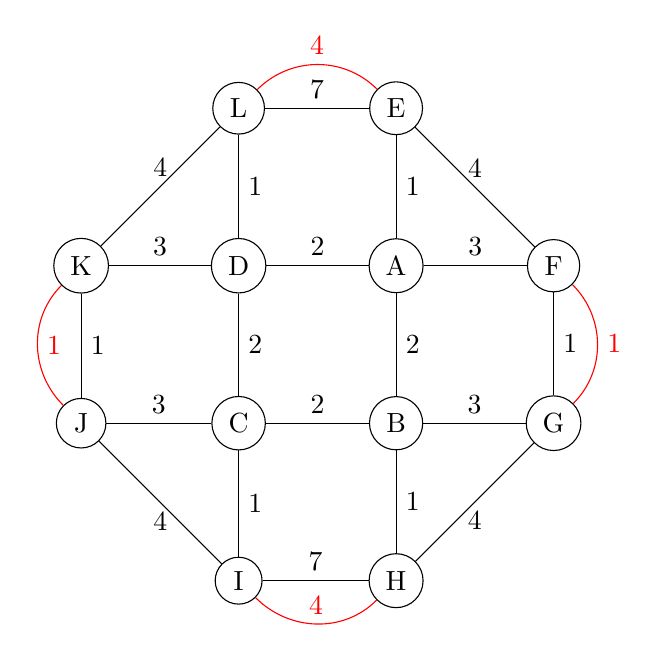
\begin{tikzpicture}
    \node[circle] (A)[draw=black] at (1,1){A};
    \node[circle] (B)[draw=black] at (1,-1){B};
    \node[circle] (C)[draw=black] at (-1,-1){C};
    \node[circle] (D)[draw=black] at (-1,1){D};
    \node[circle] (E)[draw=black] at (1,3){E};
    \node[circle] (F)[draw=black] at (3,1){F};
    \node[circle] (G)[draw=black] at (3,-1){G};
    \node[circle] (H)[draw=black] at (1,-3){H};
    \node[circle] (I)[draw=black] at (-1,-3){I};
    \node[circle] (J)[draw=black] at (-3,-1){J};
    \node[circle] (K)[draw=black] at (-3,1){K};
    \node[circle] (L)[draw=black] at (-1,3){L};

    \path (A) edge node [right] {2} (B);
    \path (B) edge node [above] {2} (C);
    \path (C) edge node [right] {2} (D);
    \path (D) edge node [above] {2} (A);
    \path (E) edge node [above] {4} (F);
    \path (F) edge node [right] {1} (G);
    \path (G) edge node [below] {4} (H);
    \path (H) edge node [above] {7} (I);
    \path (I) edge node [below] {4} (J);
    \path (J) edge node [right] {1} (K);
    \path (K) edge node [above] {4} (L);
    \path (L) edge node [above] {7} (E);
    \path (A) edge node [right] {1} (E);
    \path (A) edge node [above] {3} (F);
    \path (B) edge node [above] {3} (G);
    \path (B) edge node [right] {1} (H);
    \path (C) edge node [right] {1} (I);
    \path (C) edge node [above] {3} (J);
    \path (D) edge node [above] {3} (K);
    \path (D) edge node [right] {1} (L);
    \draw[red,out=45,in=135] (L) to node [above] {4} (E);
    \draw[red,out=-135,in=135] (K) to node [right] {1} (J);
    \draw[red,out=-45,in=45] (F) to node [right] {1} (G);
    \draw[red,out=-45,in=-135] (I) to node [above] {4} (H);
  \end{tikzpicture}
\end{center}

A présent, nous avons un graphe composé uniquement de noeuds de degré
pair. Nous savons par le théorème d'Euler, qu'il existe un parcours
fermé passant une seule fois par chaque arête. Ce parcours est le
parcours de poids minimum passant au moins une fois par chaque arête
dans le graphe de départ, son poids correspond à la somme des poids
de chaque arête dans le nouveau graphe :

\[ 7+4+1+4+7+4+1+4+1+1+3+3+1+1+3+3+2+2+2+2+\textcolor{red}{4}+\textcolor{red}{4}+\textcolor{red}{1}+\textcolor{red}{1} = 66 \]
\end{solution}

\subsection{Chemin de coût minimum}
Dans le graphe suivant, trouvez un parcours de coût minimum du sommet $1$ au sommet $7$.
Le parcours doit traverser toutes les arêtes au moins une fois.

\begin{figure}[h!]
  \begin{center}
    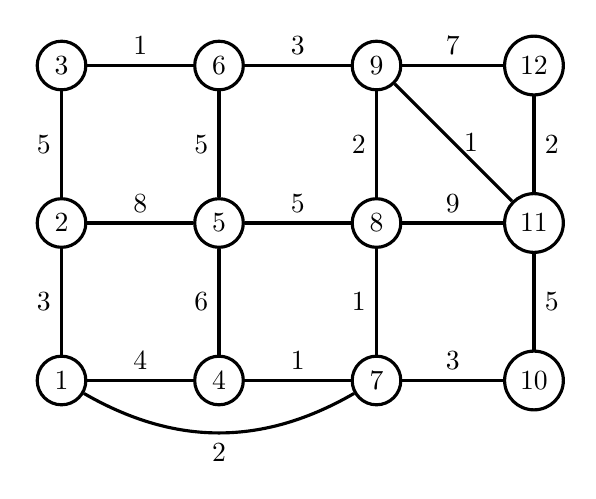
\begin{tikzpicture}[scale=2,auto,line width=.4mm]

      \path (0,0) node[draw,shape=circle] (1)  {$1$};
      \path (0,1) node[draw,shape=circle] (2)  {$2$};
      \path (0,2) node[draw,shape=circle] (3)  {$3$};
      \path (1,0) node[draw,shape=circle] (6)  {$4$};
      \path (1,1) node[draw,shape=circle] (5)  {$5$};
      \path (1,2) node[draw,shape=circle] (4)  {$6$};
      \path (2,0) node[draw,shape=circle] (7)  {$7$};
      \path (2,1) node[draw,shape=circle] (8)  {$8$};
      \path (2,2) node[draw,shape=circle] (9)  {$9$};
      \path (3,0) node[draw,shape=circle] (12) {$10$};
      \path (3,1) node[draw,shape=circle] (11) {$11$};
      \path (3,2) node[draw,shape=circle] (10) {$12$};

      \draw (1)  -- (2)  node[midway,left]  {$3$};
      \draw (2)  -- (3)  node[midway,left]  {$5$};
      \draw (6)  -- (5)  node[midway,left]  {$6$};
      \draw (5)  -- (4)  node[midway,left]  {$5$};
      \draw (7)  -- (8)  node[midway,left]  {$1$};
      \draw (8)  -- (9)  node[midway,left]  {$2$};
      \draw (12) -- (11) node[midway,right] {$5$};
      \draw (11) -- (10) node[midway,right] {$2$};
      \draw (1)  -- (6)  node[midway,above] {$4$};
      \draw (2)  -- (5)  node[midway,above] {$8$};
      \draw (3)  -- (4)  node[midway,above] {$1$};
      \draw (4)  -- (9)  node[midway,above] {$3$};
      \draw (5)  -- (8)  node[midway,above] {$5$};
      \draw (6)  -- (7)  node[midway,above] {$1$};
      \draw (7)  -- (12) node[midway,above] {$3$};
      \draw (8)  -- (11) node[midway,above] {$9$};
      \draw (9)  -- (10) node[midway,above] {$7$};
      \draw (9)  -- (11) node[midway,above,right] {$1$};
      \draw (1) to[bend right] node[midway,below] {$2$} (7);

    \end{tikzpicture}
  \end{center}
\end{figure}

\begin{solution}
Le raisonnement est similaire à celui de l'exercice 5. Nous devons
trouver un chemin de coût minimum du sommet 1 au sommet 7. Le chemin
doit traverser toutes les arêtes au moins une fois. 

Le cas idéal est celui d'un parcours eulérien du sommet 1 au sommet 7 (dans ce cas
on ne passe qu'une seule fois par chaque arête). Pour avoir un parcours
eulérien, il faut que les sommets de départ et d'arrivée (sommet 1
\& 7) soient de degré impair. 

Le sommet 1 est bien de degré impair,
par contre le sommet 7 est de degré pair, il faudra donc ajouter une
arête incidente à ce sommet. De plus, tous les autres sommets doivent
avoir un degré pair. Par conséquent, il faut ajouter une arête aux
sommets 2, 6 \& 4. Nous avons 4 sommets (2, 4, 6 \& 7) auquel il faut
ajouter une arête. 

Nous les regroupons par paire afin d'avoir le plus
court chemin possible entre chaque paire. Ce qui nous donne 4 avec
7 et 2 avec 6. A présent, il ne nous reste plus qu'à ajouter une arête
entre chaque paire de sommets, le poids de la nouvelle arête correspond
aux poids du parcours minimum entre les 2 sommets. L'arête entre 4
et 7 aura un poids 1, l'arête entre 2 et 6 aura un poids 6. 

A présent, notre graphe a 2 sommets de degré impair, il existe donc un parcours
eulérien entre ces 2 sommets. Ce parcours est le parcours de poids
minimum du sommet 1 au sommet 7 passant au moins une fois par chaque
arête dans le graphe de départ, sont poids vaut 79.
\end{solution}

\subsection{Postier chinois dans l'hypercube} Résolvez le problème du postier chinois sur l'hypercube de dimension $k$.
